\subsubsection{RASIMAS}
\label{art:rasimas}

\todo{ es importante que describas la RA y la Radiología diagnostica en el estado del arte. Deben ir los pasos detallados del procedimiento. Pon alguna cita en el estado del arte. Por ejemplo, el CV de RA de Cork. Esto luego lo usaras en el courseware}

La \acl{RA}(\acs{RA}) guiada por \acl{US}(\acs{US}) representa una alternativa a la estimulación eléctrica. Las ventajas de utilizar una imagen de \ac{US} solventa las debilidades de la técnica tradicionalmente prácticada. La principal ventaja es la posibilidad de confirmar la propagación del anestésico alrededor del nervio objetivo. Además de la posibilidad de observar la aguja y el nervio, la imagen revela todas las estructuras internas como fascias, pleura, e incluso tejidos delicados como los vasos sanguíneos. 

\begin{figure}[h]
   \centering
    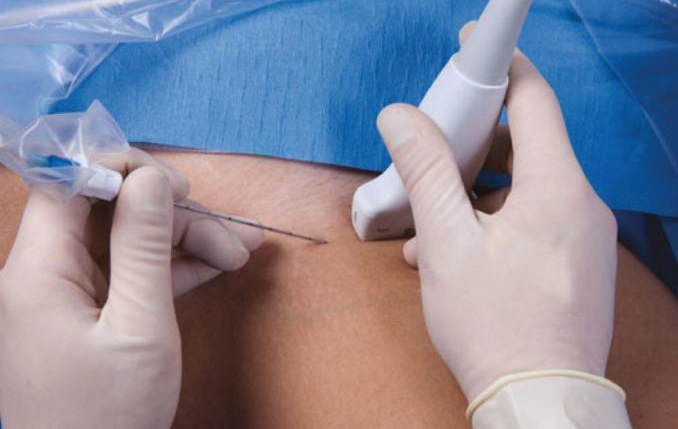
\includegraphics[width=0.5\textwidth]{IMG/RAUS.png}
    \caption{ Anestesia regional guiada por \acl{US}}
   \label{fig:raus}
\end{figure}

La ejecución de este procedimiento no es sencillo para aquellos profesionales de anestesiología que no están familiarizados con las técnicas de \ac{US}. Además de los conocimientos teóricos, los profesionales deben entrenar sus habilidades no cognitivas. Estos entrenamientos habitualmente se practican con paciente reales, con la utilización de cadáveres\cite{Tsui2007} o el uso de \emph{fantomas}\cite{phantomra}. La incorporación de un simulador en el entrenamiento del procedimiento ayudará a solventar las limitaciones de los entrenamientos clásicos al ser más barato, repetible y seguro.

El proyecto \ac{RASimAs} tiene como objetivo \new{el} de facilitar el entrenamiento y la práctica de la \ac{RA} con la ayuda de un simulador (\ac{RASim}) y un asistente (\ac{RAAs}).
Para que sea utilizado en el mayor número de sitios posibles (hospitales, universidades y colegios profesionales) se debe proporcionar una herramienta de entrenamiento que sea barata, fácil de usar, robusta y que necesite poco mantenimiento.
Estas herramientas están dirigidas para diferentes perfiles de usuarios.  Tanto estudiantes como profesionales que están empezando a realizar el procedimiento, el simulador les proporcionará un método de entrenamiento con el que mejorar sus habilidades cognitivas y propioceptivas. A su vez, este proyecto también está orientado para profesionales anestesistas que han estado alejados de la práctica del procedimiento y quieran retomar la actividad.
Los objetivos principales del simulador \ac{RASim} son los siguientes:
\begin{enumerate}
    \item Un estudiante de \new{anestesista} \del{anestesista} adquiera y desarrolle las habilidades cognitivas y no cognitivas que le permitan ejecutar un bloque de nervio guiado por \ac{US} empezando por el bloqueo del nervio femoral y siguiendo con las siguientes localizaciones.
    \item Permitir a un anestesista retomar y practicar las habilidades necesarias para realizar el procedimiento de forma segura y satisfactoria.
    \item Recuperar y medir métricas de rendimiento al realizar el procedimiento en el simulador. 
    \item Permitir a un supervisor revisar las métricas registradas por los usuarios del simulador a través del tiempo
\end{enumerate}



Según (entregable 2.1 \cite{rasimasweb}), el procedimiento de \ac{RA} guiado por \ac{US} se puede definir con los siguientes bloques:
\begin{enumerate}
    \item Exploración (\emph{Scout Scan}): El profesional configura y explora con la sonda de \ac{US} la zona del paciente con el objetivo de identificar el nervio, la arteria principal y las demás estructuras importantes (figura \ref{fig:scoutscan}). 
\begin{figure}[th]
   \centering
    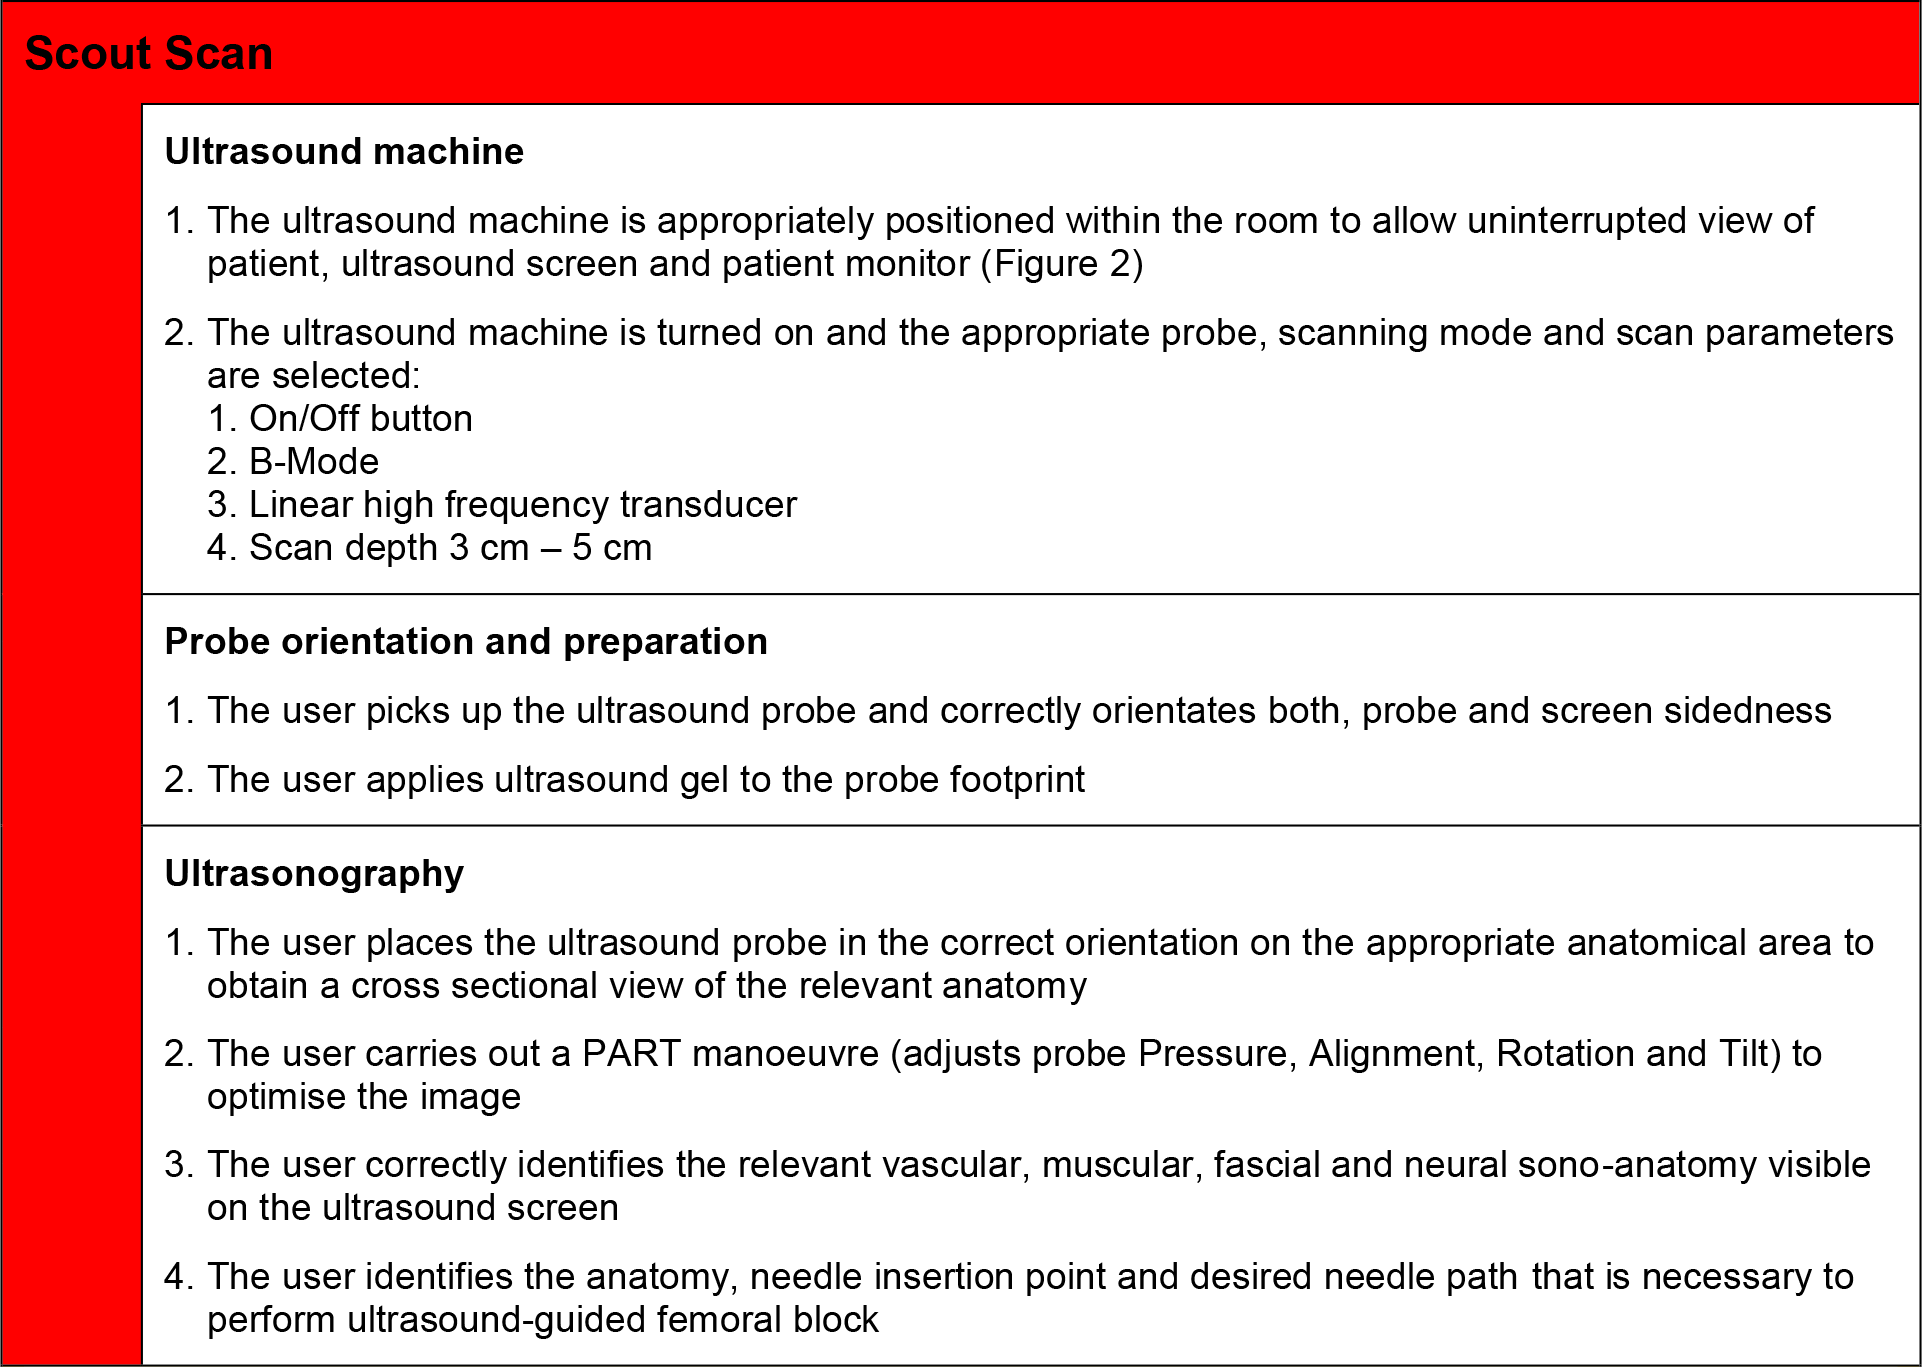
\includegraphics[width=0.9\textwidth]{IMG/scoutscan.png}
    \caption{Tareas del bloque de exploración }
   \label{fig:scoutscan}
   
\end{figure}
\todo{ Las imágenes se ven fatal, las paso a word, word a pdf y las pongo en el anexo? puedo citarlas también en los resultados}
    \item Guiado de la aguja (\emph{Needle Guidance}): A partir de que se ha interpretado la imagen de \ac{US}, el profesional guía la aguja a través de la anatomía hasta el nervio (figura \ref{fig:needleguidance}).  
    \begin{figure}[th]
   \centering
    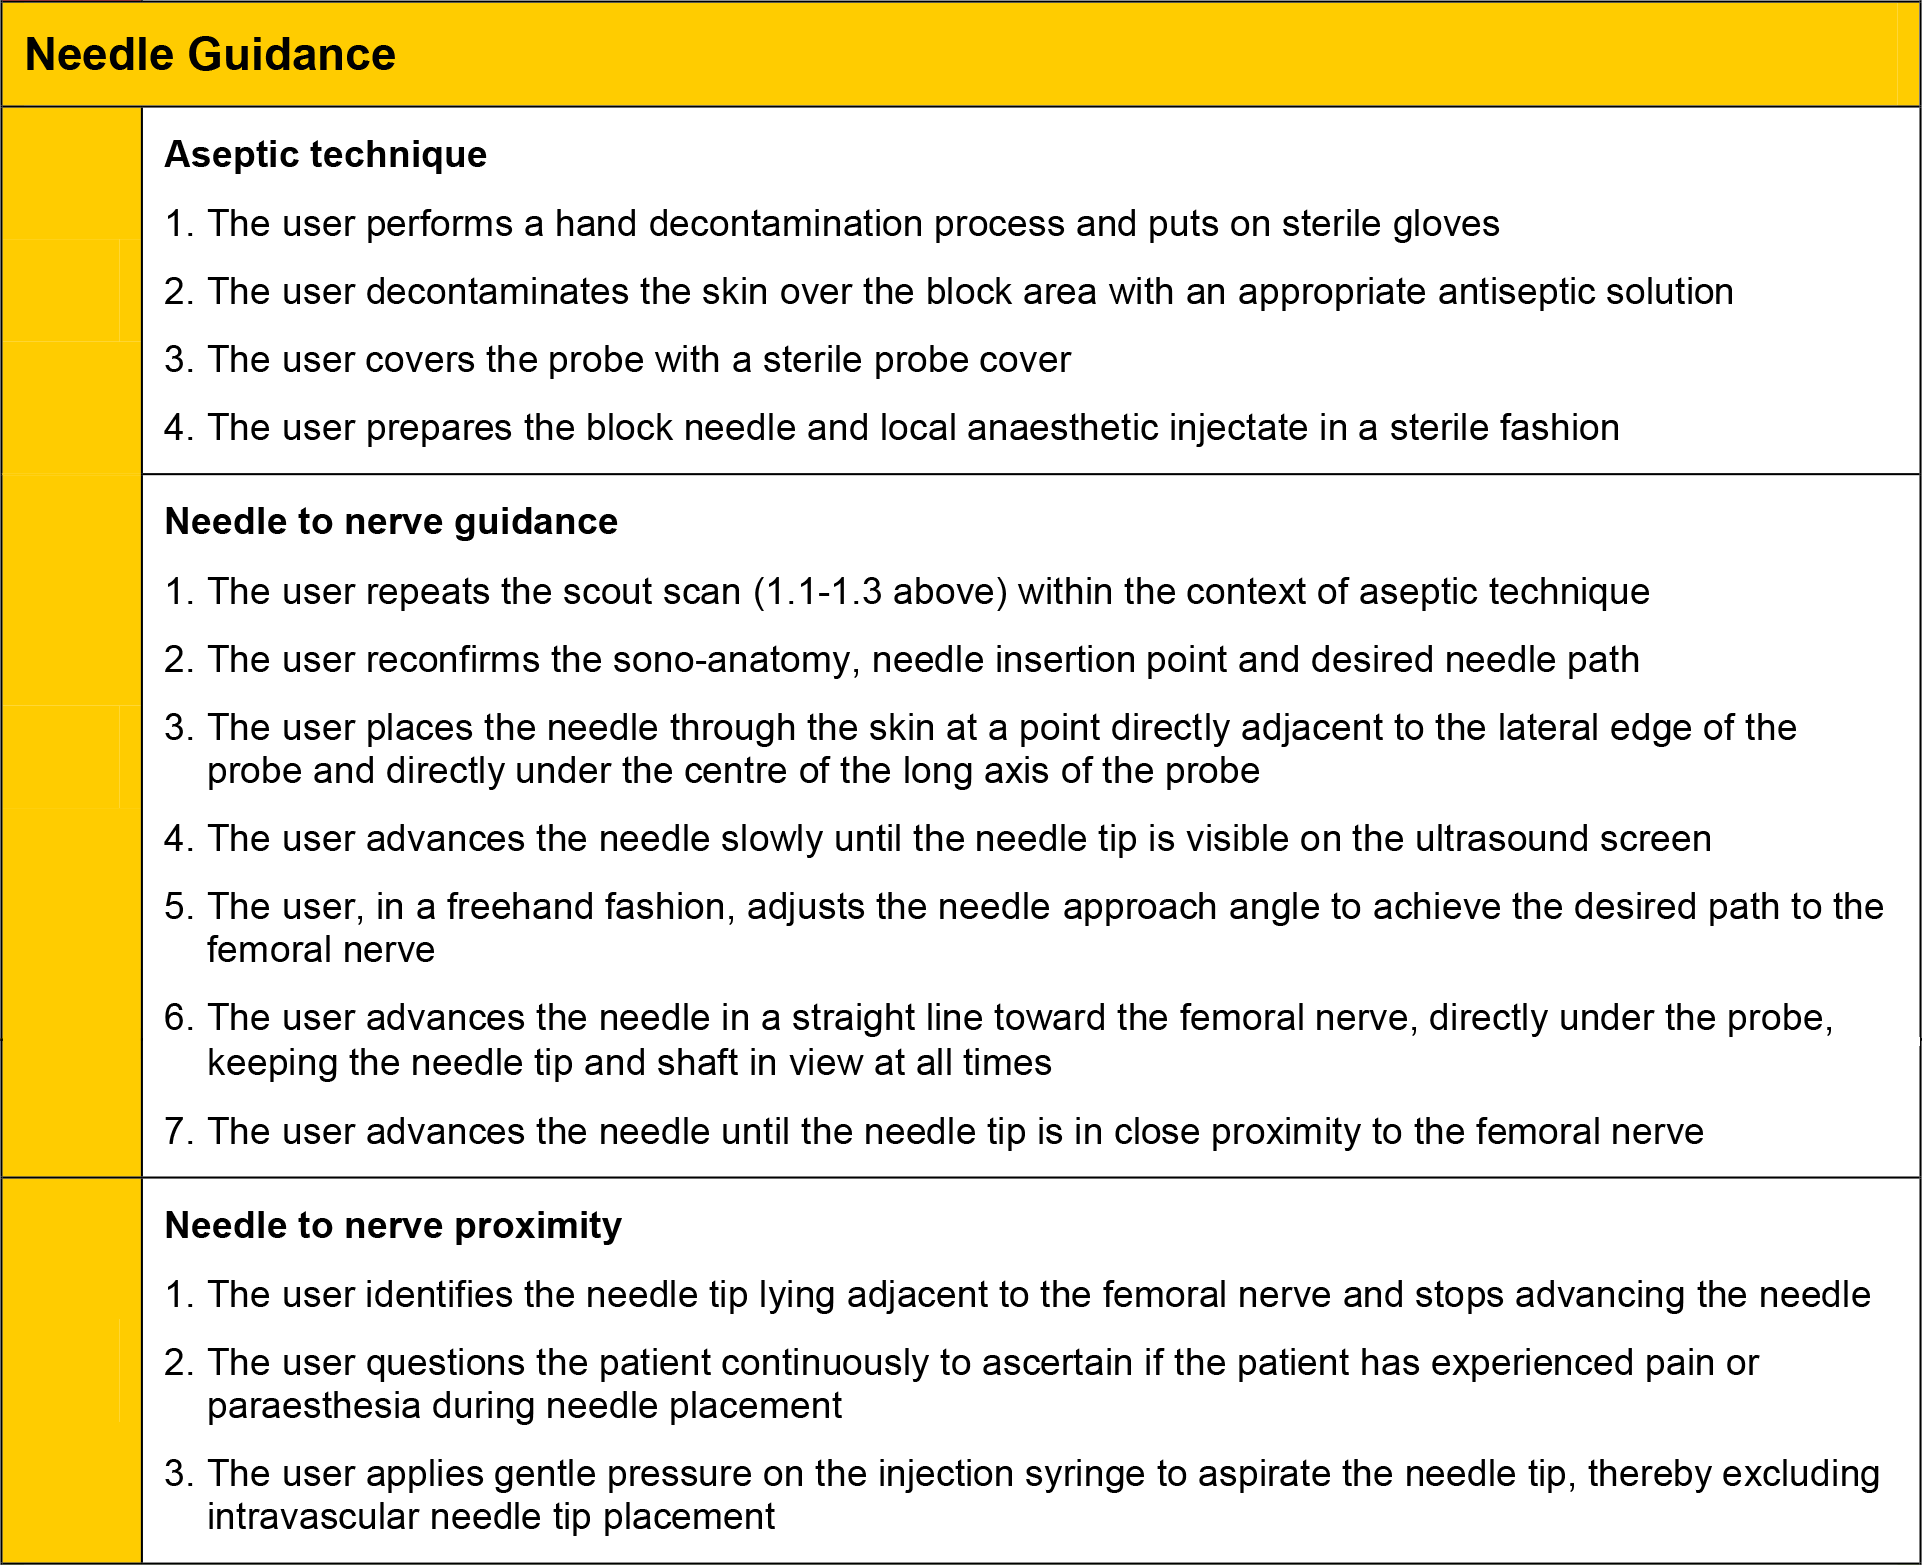
\includegraphics[width=0.9\textwidth]{IMG/needleguidance.png}
    \caption{Tareas del bloque de guiado de la aguja. }
   \label{fig:needleguidance}
\end{figure}
    \item Inyección (\emph{Injection}): El médico libera el bolo y confirma la correcta realización del bloqueo del nervio (figura \ref{fig:injection}). 
    \begin{figure}[th]
   \centering
    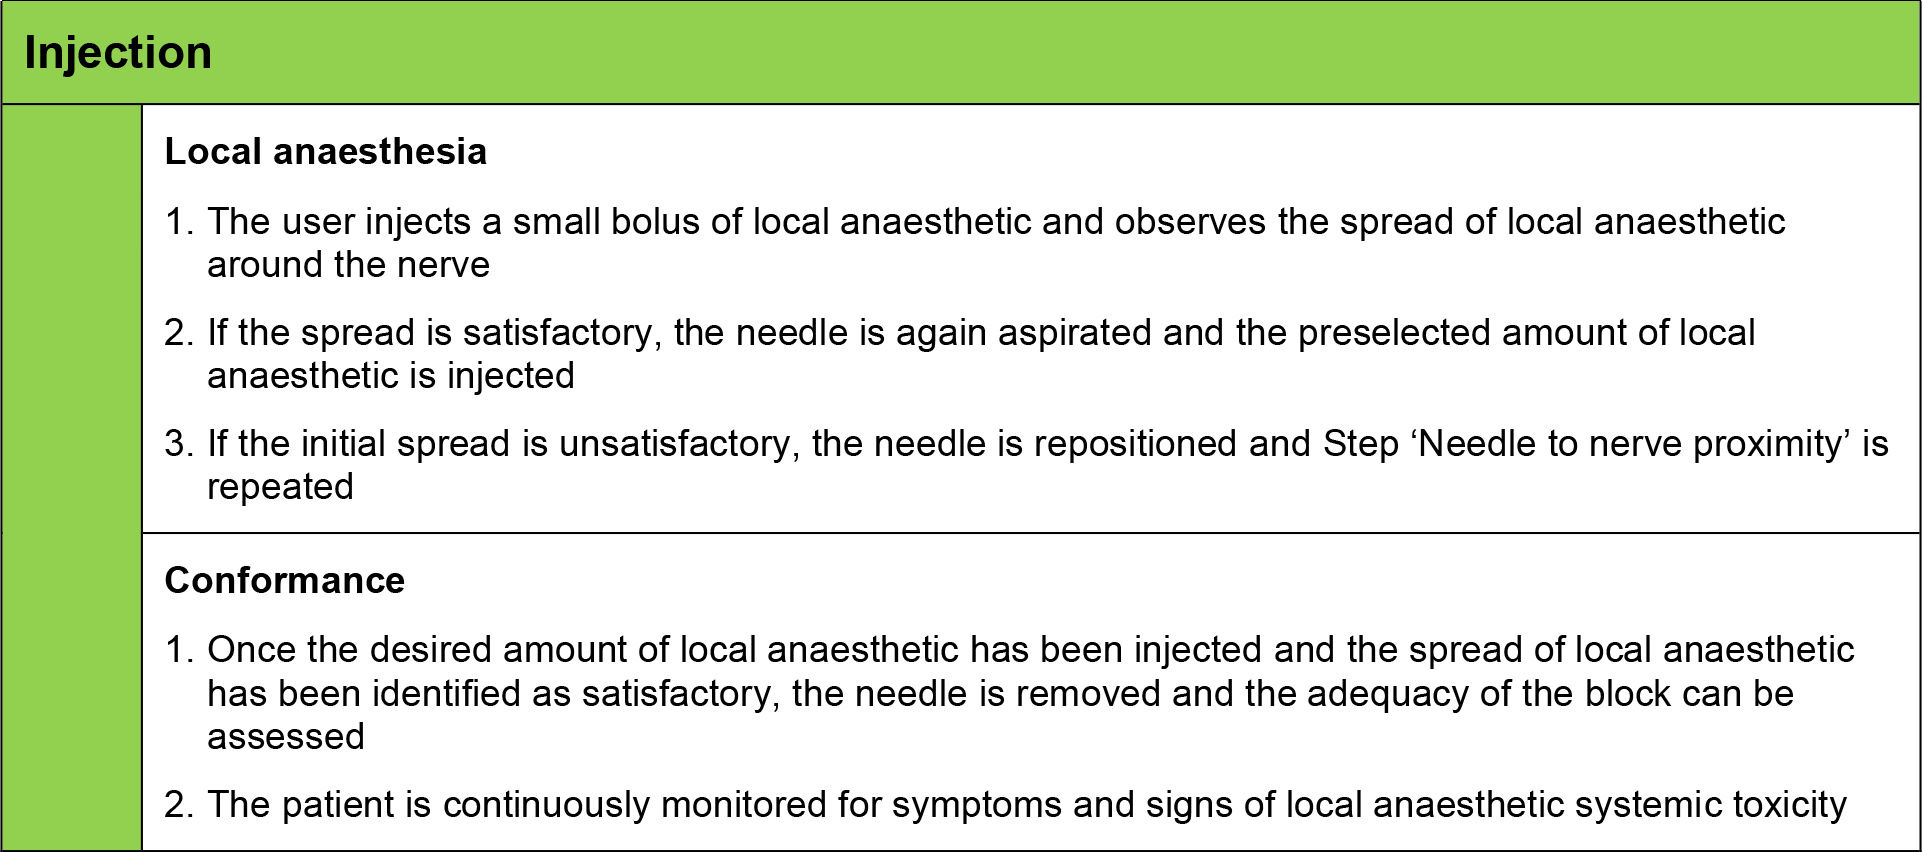
\includegraphics[width=0.9\textwidth]{IMG/injection.png}
    \caption{ Tareas del bloque de inyección.}
   \label{fig:injection}
\end{figure}
\end{enumerate}

Con el objetivo de explicar detalladamente cada bloque, se resumirá a continuación el procedimiento completo:

El anestesista deberá posicionarse en la sala de tal forma que su ángulo de visión permita observar el paciente, y el monitor de \ac{US} y de las constantes vitales sin mover la cabeza (figura \ref{fig:roomplace}). El médico configurará el equipo de \ac{US} con los valores apropiados, y explorará la zona anatómica con la sonda. Para conseguir una imagen adecuada para identificar los tejidos, se procederá a la maniobra PART (del inglés \emph{Pressure, Alignment, Rotation and Tilt}) que permite colocar correctamente la sonda de \ac{US} para asegurar una buena imagen donde se puedan localizar todas las estructuras importantes. Una vez el nervio esté localizado, el médico introducirá la aguja en plano\footnote{La aguja se introduce en paralelo con la proyección ultrasonográfica para que quede totalmente visible en la imagen.} con la sonda de \ac{US}, permitiendo así su visualización en la imagen y la dirigirá hasta la proximidad del nervio. Es entonces cuando, antes de inyectar el bolo, deberá aspirar primero para comprobar que la punta de la aguja no se encuentre dentro de un vaso sanguíneo y pueda causar toxicidad sistémica \footnote{El anestésico se distribuirá por los vasos sanguíneos.}. Una vez comprobado, a continuación solo se distribuirá una pequeña cantidad para asegurarse de la localización de la aguja y por último se liberará el bolo completamente. El profesional deberá confirmar que el bloqueo ha sido satisfactorio y comprobará cualquier síntoma de malestar en el paciente.


\begin{figure}[th]
   \centering
    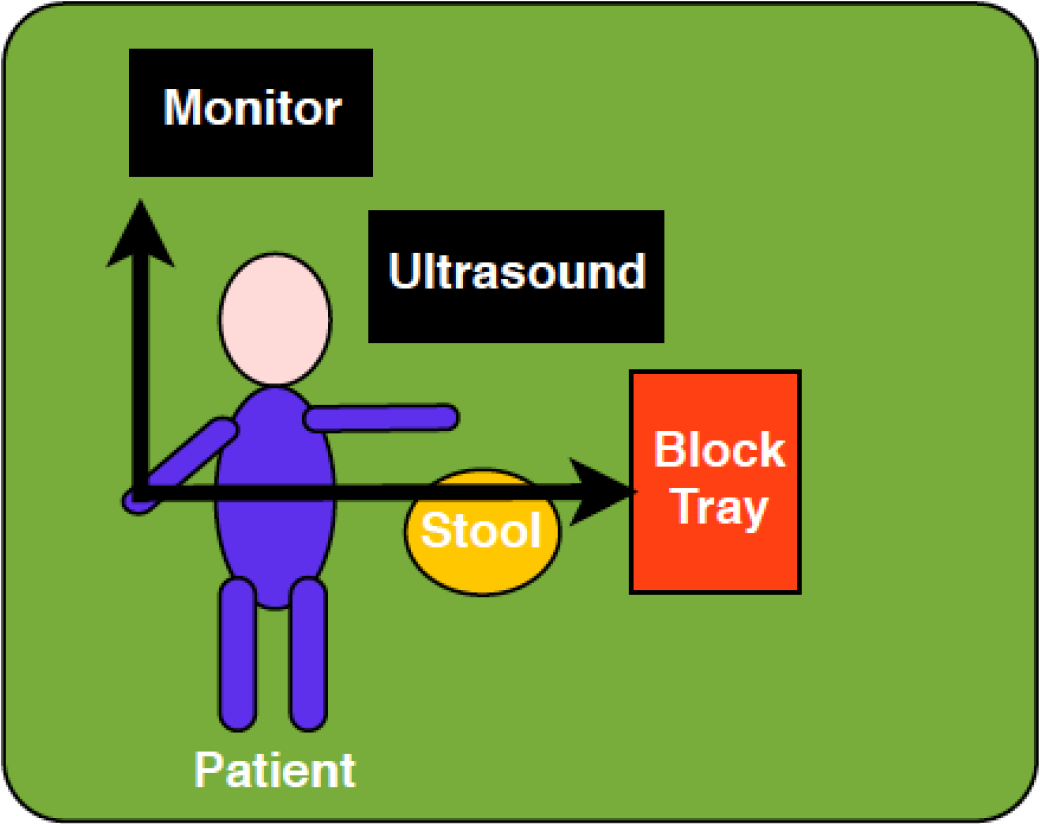
\includegraphics[width=0.5\textwidth]{IMG/roomplacement.png}
    \caption{ }
   \label{fig:roomplace}
\end{figure}




%\subsubsection{Objetivos del simulador}


% 6.1.3 Principles of use
% 1. RASim must be contextually relevant and function within the existing or evolving regional
% anaesthesia curriculum
% 2. RASim training must be based upon appropriately detailed characterised procedures
% 3. RASim training must allow the development of relevant procedural skills and associated
% clinical decision making
% 4. RASim training must never allow the development of procedural skill relevant only within
% the simulation environmentRASim training should allow performance related feedback, repeated practice and
% performance tracking and progression over time each based on precisely defined metrics
% 6. RASim based training programmes must have a defined beginning and end (entry and
% exit) constituting proficiency based progression for defined applications e.g. independent
%practice , supervised practice

